W celu zapewnienia optymalnej czytelności oraz precyzyjnego odwzorowania cyklu życia domeny biznesowej, ostateczny model wypracowany podczas sesji Event Stormingowej został zaprezentowany w formie podziału na sekwencyjne etapy. Należy jednak stanowczo podkreślić, że \textbf{przedstawione na kolejnych schematach fazy nie są odizolowanymi procesami, lecz stanowią jeden, spójny i chronologiczny ciąg zdarzeń biznesowych} modelowanego systemu DMS.

Podział na odrębne grafiki (Etapy 1-5 oraz gałąź asynchroniczną) podyktowany jest wysoką złożonością domeny i naturalnym przechodzeniem odpowiedzialności pomiędzy poszczególnymi Kontekstami Ograniczonymi (Sprzedaż, Katalog, Finansowanie, Fakturowanie oraz Inwentarz).

Całościowy przepływ (\textit{Domain Flow}) realizowany jest w sposób ciągły:
\begin{itemize}
    \item \textbf{Etap 1 i 2} obrazują początek osi czasu: od pierwszej interakcji klienta w konfiguratorze, aż po wygenerowanie wiążącego zamówienia i kluczowe rozwidlenie ścieżki płatności (gotówka lub finansowanie zewnętrzne).
    
    \item \textbf{Etap 3 i 4} to płynna kontynuacja procesu, w której na podstawie gwarancji finansowej z poprzednich kroków, system uruchamia operacje magazynowo-logistyczne (rezerwacja na placu lub zlecenie do fabryki po opłaceniu zadatku), kończąc się wystawieniem faktury i pełnym rozliczeniem.
    
    \item \textbf{Etap 5} stanowi zwieńczenie głównego strumienia transakcji, w którym w pełni opłacony i gotowy logistycznie pojazd jest fizycznie wydawany klientowi, zamykając cykl życia zamówienia.
    
    \item Dopełnieniem całości jest wyodrębniona \textbf{Gałąź asynchroniczna}, która działa w tle jako mechanizm zabezpieczający (wyzwalany upływem czasu), mogący w dowolnym momencie przerwać główny ciąg w przypadku braku uregulowania należności przez klienta.
\end{itemize}

Takie sekwencyjne podejście pozwala śledzić stan nadrzędnych agregatów (takich jak \textit{Zamówienie} czy \textit{Egzemplarz Pojazdu}) przechodzących przez kolejne maszyny stanów w ramach całego zintegrowanego procesu salonu samochodowego.

\begin{figure}[H]
    \centering
    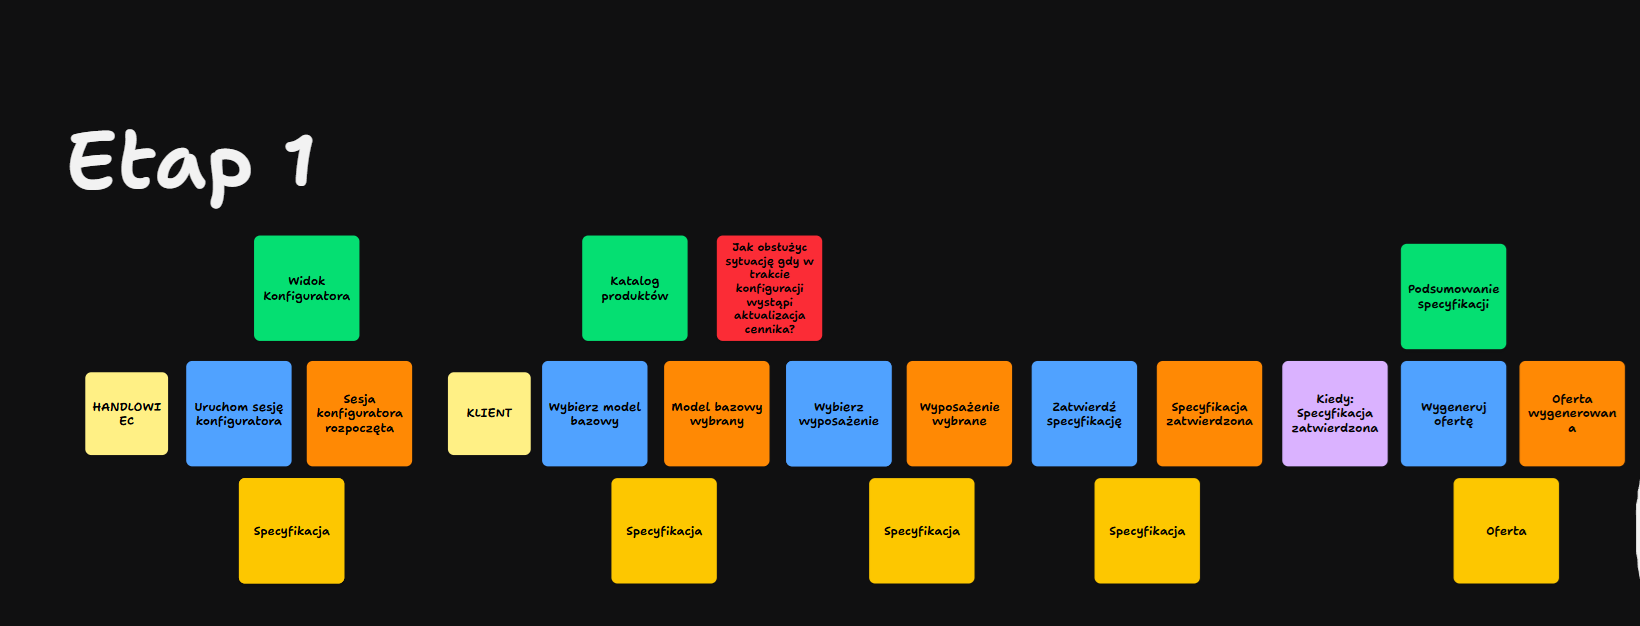
\includegraphics[width=\textwidth]{media/event-storming-poprawiony/Event_stormingE1.png}
    \caption{Etap 1: Konfiguracja pojazdu oraz wygenerowanie oferty}
    \label{fig:es_etap1}
\end{figure}

\begin{figure}[H]
    \centering
    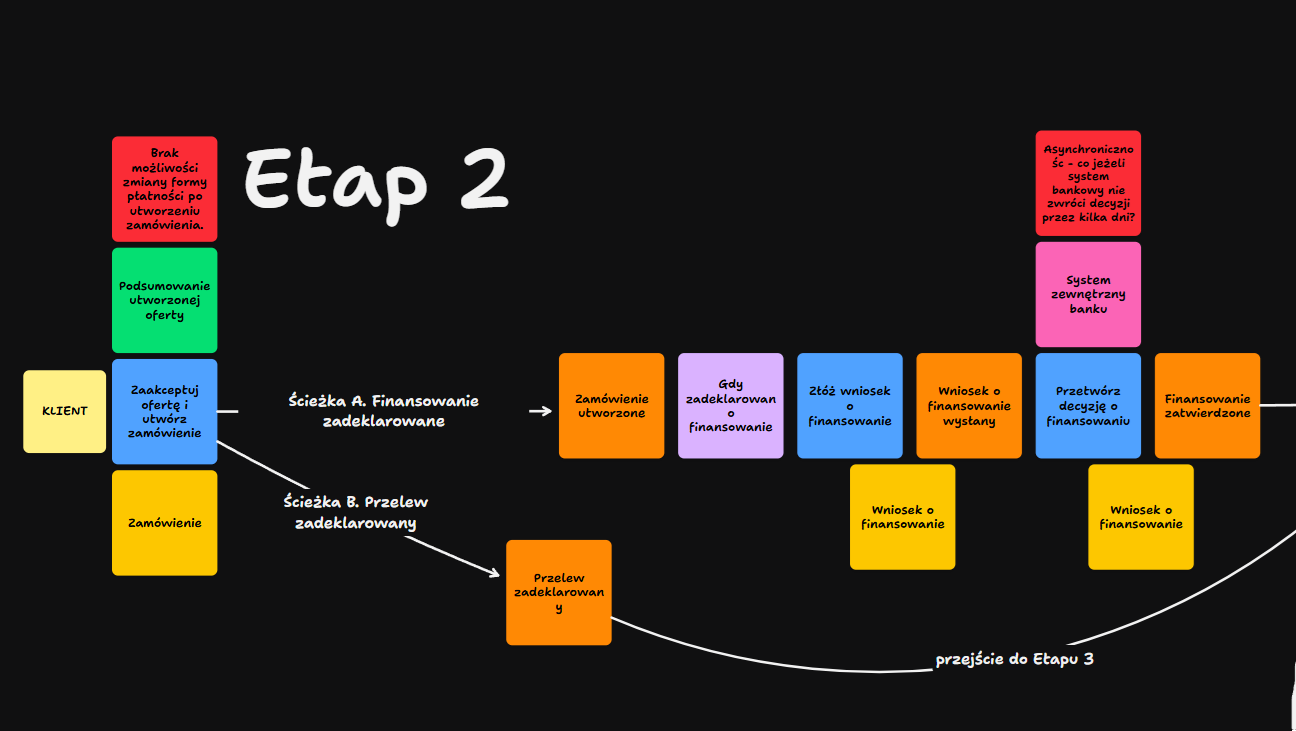
\includegraphics[width=\textwidth]{media/event-storming-poprawiony/Event_stormingE2.png}
    \caption{Etap 2: Utworzenie zamówienia i wybór ścieżki płatności}
    \label{fig:es_etap2}
\end{figure}

\begin{figure}[H]
    \centering
    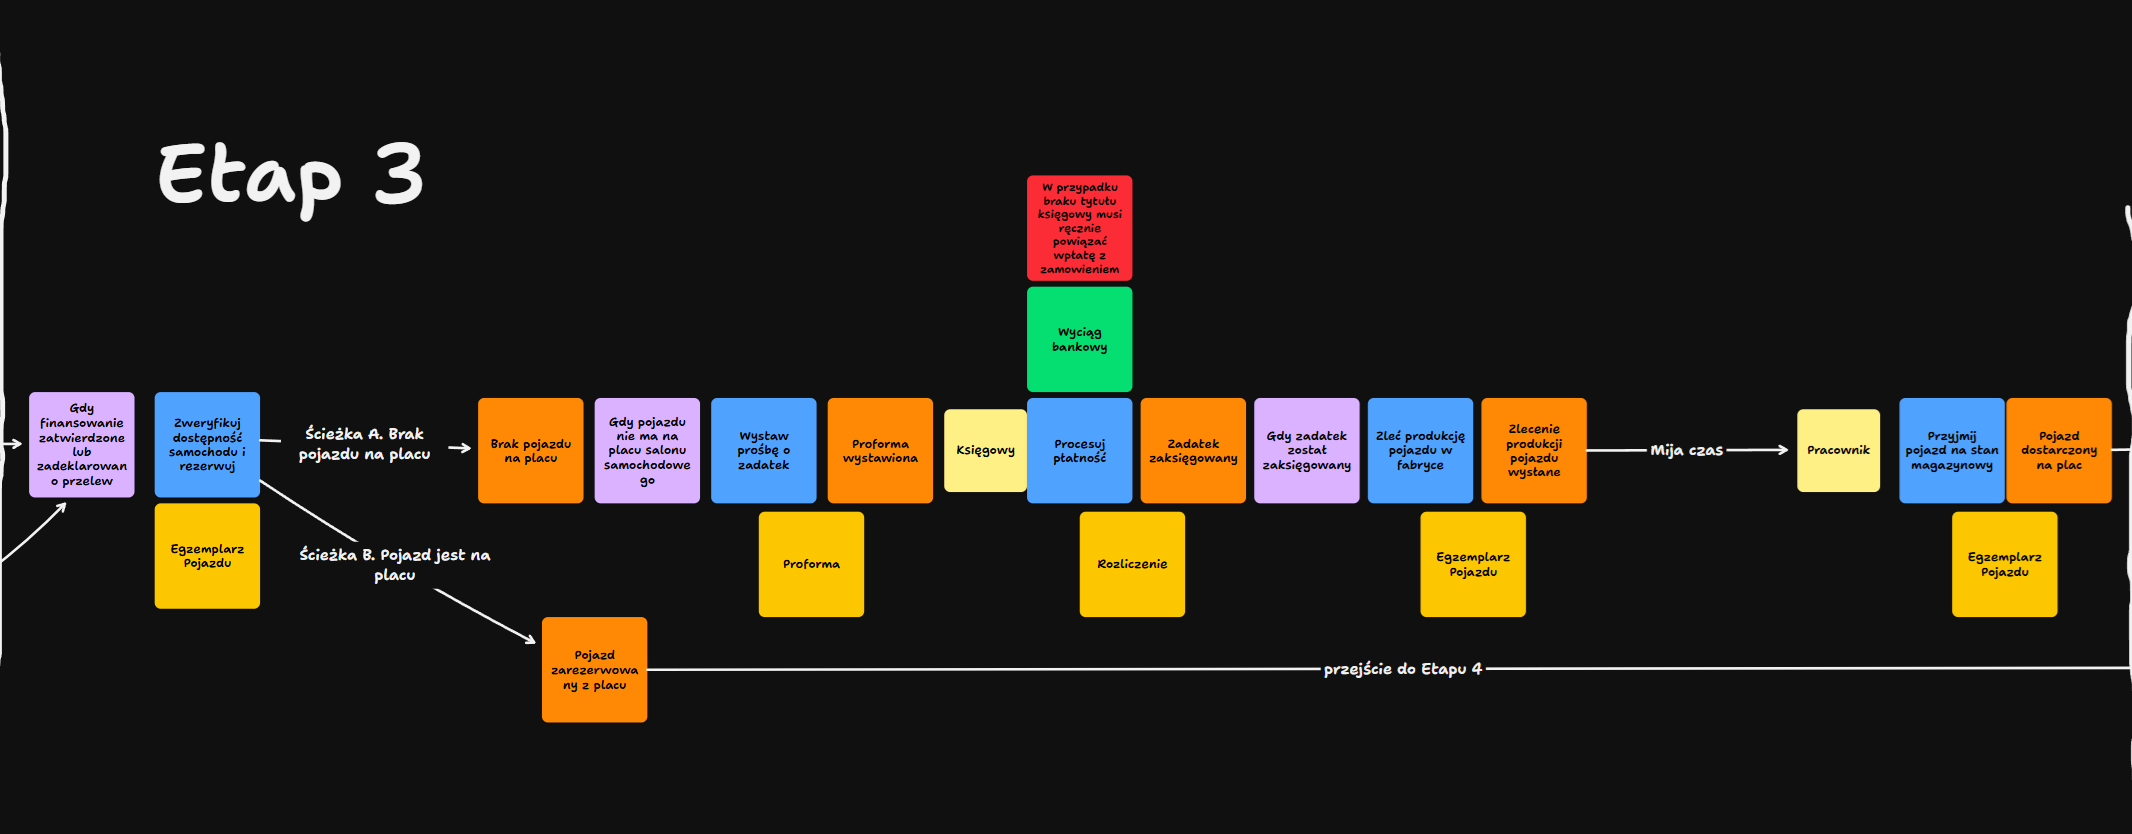
\includegraphics[width=\textwidth]{media/event-storming-poprawiony/Event_stormingE3.png}
    \caption{Etap 3: Weryfikacja placu, proces bankowy oraz zlecenia fabryczne}
    \label{fig:es_etap3}
\end{figure}

\begin{figure}[H]
    \centering
    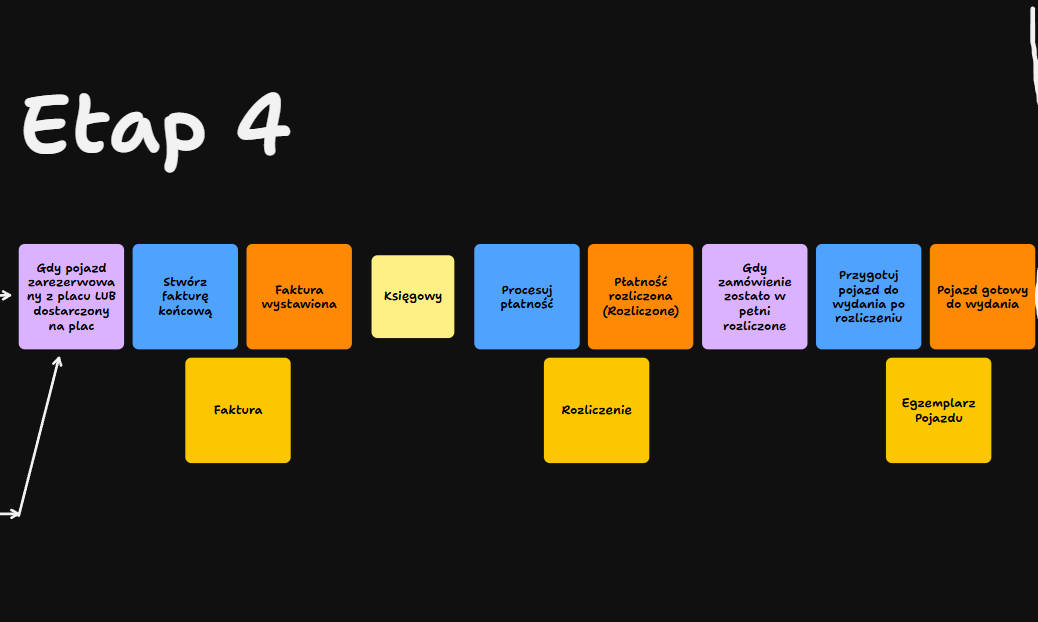
\includegraphics[width=\textwidth]{media/event-storming-poprawiony/Event_stormingE4.png}
    \caption{Etap 4: Fakturowanie końcowe i pełne rozliczenie zamówienia}
    \label{fig:es_etap4}
\end{figure}

\begin{figure}[H]
    \centering
    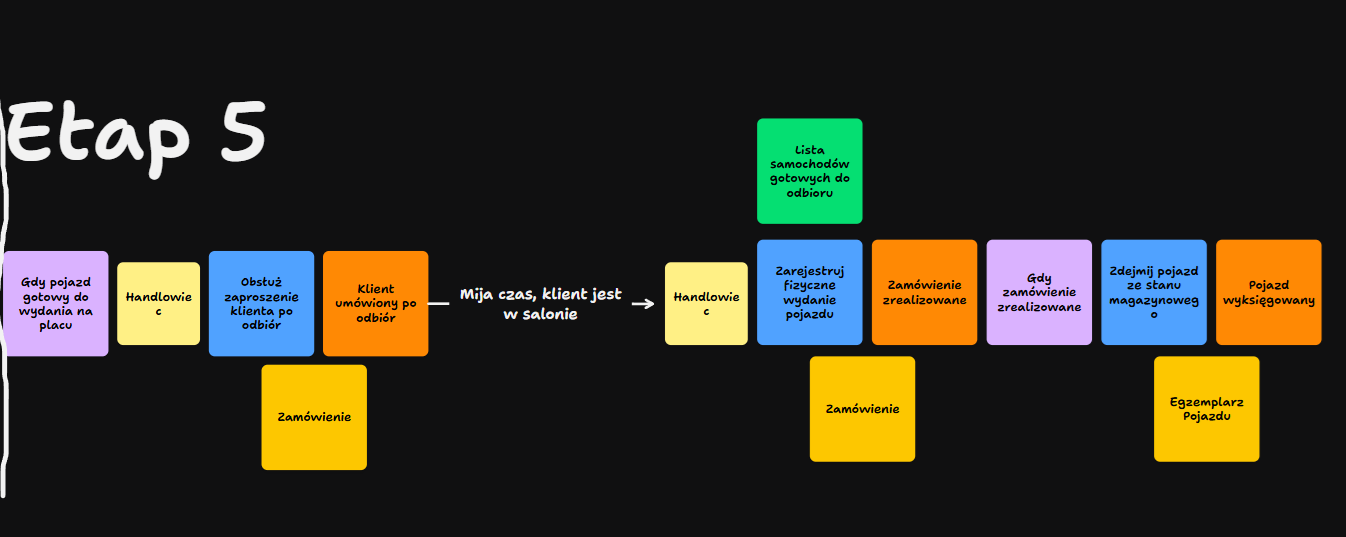
\includegraphics[width=\textwidth]{media/event-storming-poprawiony/Event_stormingE5.png}
    \caption{Etap 5: Fizyczne wydanie pojazdu i wyksięgowanie ze stanu magazynowego}
    \label{fig:es_etap5}
\end{figure}

\begin{figure}[H]
    \centering
    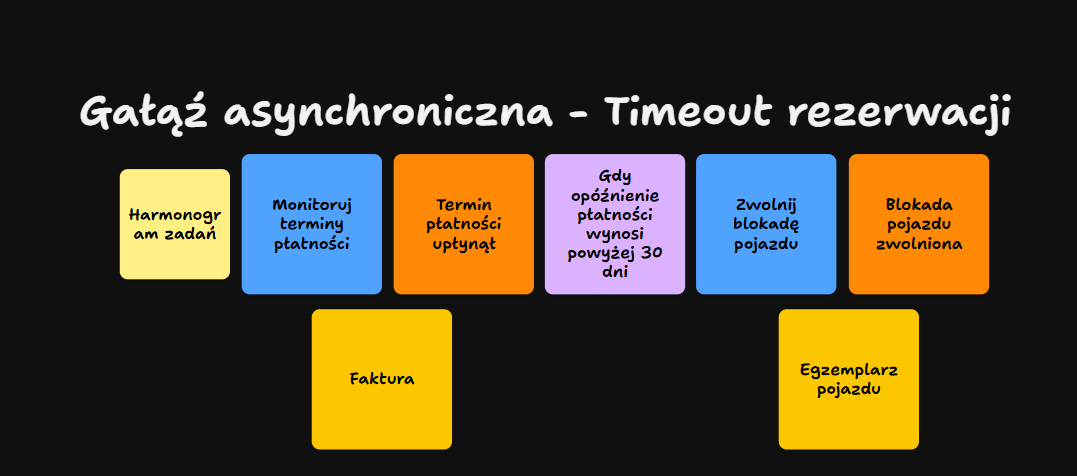
\includegraphics[width=\textwidth]{media/event-storming-poprawiony/Event_stormingE6.png}
    \caption{Gałąź asynchroniczna: Monitorowanie terminów płatności i zwolnienie blokady (Timeout)}
    \label{fig:es_etap6}
\end{figure}